\documentclass[11pt,a4paper]{article}

%\renewcommand{\section}{\section{\bold{#1}}

\newcommand{\blankpage}{
\newpage
\thispagestyle{empty}
\mbox{}
\newpage
}

\usepackage[colorlinks=false]{hyperref}
\hypersetup{%
  colorlinks = true,
  linkcolor  = black
}
\usepackage{geometry}
\usepackage{url}
\usepackage{booktabs}

\usepackage{graphicx,subcaption}
\usepackage{xspace}
\usepackage[export]{adjustbox}

\usepackage{comment}
\usepackage{caption}


\usepackage[belowskip=-15pt,aboveskip=0pt]{caption}
% maths
\usepackage{bm}
\usepackage{xspace}
\usepackage{amsmath} % Required for \ln


\makeatother
\newcommand{\farg}[1]{\ensuremath{\textbf{arg}_{#1}}\xspace}

% % Fonts
\usepackage{times}
\usepackage[T1]{fontenc}

\usepackage{float}

\onecolumn

\def\course{Sistemas de Computação Móvel e Ubíqua }
\def\coursePT{Sistemas de Computação Móvel e Ubíqua }

\def\titulo{\course{}}
\title{\titulo}

\def\data{\today}
\date{\data}

% Set your name here
\def\name{José Costa, Rodrigo Albuquerque e Rafael Mira}
\def\studentNumber{62637, 70294 e 59243}
\def\institution{Faculdade de Ci{\^e}ncias e Tecnologia\\
Universidade NOVA de Lisboa}

\author{\name\\\studentNumber\\ \institution}

% The following metadata will show up in the PDF properties
\hypersetup{
  colorlinks = true,
  urlcolor = black,
  pdfauthor = {\name},
  pdftitle = {\course: Relatório},
  pdfsubject = {\course},
  pdfpagemode = UseNone
}
\begin{comment}
\geometry{
  body={6.5in, 9.0in},
  left=1.0in,
  top=1.0in
}
\end{comment}

\geometry{
  left=0.75in,  % Adjust this value to change the left margin
  right=0.75in, % Adjust this value to change the right margin
  top=1.0in,
  bottom=1.0in,
}

% Customize page headers
\pagestyle{myheadings}
\markright{\course}
\thispagestyle{empty}

% Custom section fonts
\usepackage{sectsty}

\usepackage{amsmath}

\sectionfont{\rmfamily\mdseries\Large\textbf}
\subsectionfont{\rmfamily\mdseries\itshape\large}

\begin{document}

\pagenumbering{arabic} 

\maketitle

\section{Introduction}
The Smart Aquarium is an IoT-powered system designed to simplify the care and maintenance of multiple aquariums, such as those found in pet shops or colectors setups. By continuously monitoring environmental conditions and responding automatically to any undesirable changes, the system helps ensure a healthy and stable habitat for aquatic life with minimal manual effort.

It is componsed of several sensors and actuators, complemented by a mobile application that enables users to remotely monitor and manage their aquariums, offering convenience and control.

\section{General Overview}

Each user has their own aquarium and a mobile application. A user can manage multiple aquariums.

The system supports multiple clients. An aquarium owner can share visibility of their aquarium with other users.

The system uses a Spring Boot backend running on a server that communicates with both the mobile application and the ESP32 microcontroller.

Each aquarium requires one microcontroller.

\begin{itemize}
    \setlength\itemsep{0.1em}
    \item TDS Sensor
    \item Temperature Sensor
    \item pH Sensor
    \item Ultrasonic Sensor
    \item LDR Sensor
\end{itemize}

The actuators are:

\begin{itemize}
    \setlength\itemsep{0.1em}
    \item OLED Display
    \item Water Pump
    \item Buzzer
\end{itemize}

Each microcontroller must be connected to at least one of the supported sensors and one of the actuators.

After the initial setup is complete, sensor readings are displayed on the OLED screen.

If any reading exceeds the user-defined thresholds, the buzzer will alert the user.

To refill the aquarium, the user can activate the water pump either when the TDS threshold is exceeded or manually through a button in the mobile application.

\section{System Architecture}

\begin{figure}[H]
  \centering
  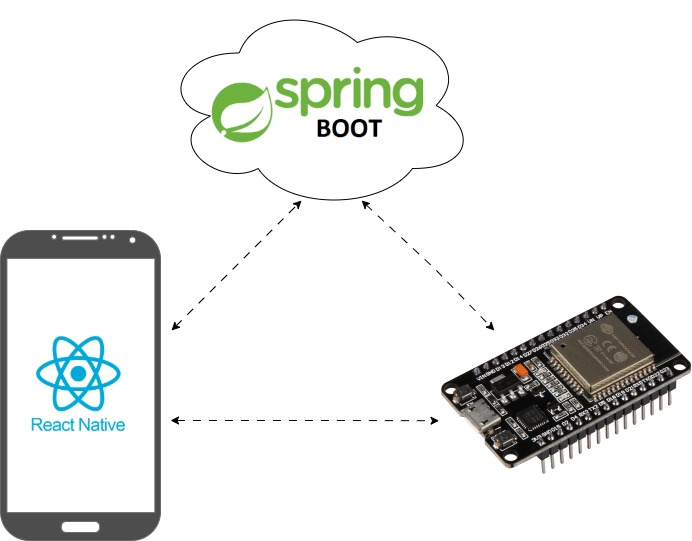
\includegraphics[width=0.5\columnwidth]{Images/Layout.jpg}
  \setlength{\belowcaptionskip}{0pt}
  \caption{System Architecture}
  \label{fig:components}
\end{figure}

\subsection{Hardware Layer}

This layer is centered around microcontrollers (e.g., ESP32) connected to a set of environmental sensors and actuators. Each microcontroller gathers sensor data and communicates with the backend server to report readings and receive control commands.
In our setup, two ESP32 devices are deployed in parallel, each managing its own set of sensors and actuators while communicating with the rest of the system over the network.

For initial setup, the system uses the Bluetooth Low Energy (BLE) protocol to pair with the user's smartphone and receive Wi-Fi credentials. BLE was chosen for its low power consumption and wide support on mobile devices. Once connected to the internet, the microcontrollers communicate with the backend server, registering their unique MAC address to an aquarium.

\subsection{Backend Server}

The backend layer is implemented using Spring Boot and serves as the central hub for communication between the microcontrollers and the mobile application. It exposes a set of secure RESTful APIs to receive sensor data from the hardware, process control commands from the mobile app, and coordinate system behavior. A MySQL database is used to store historical sensor readings and device states.

In the current setup, the backend server is deployed in a Docker container running on a local server. To enable remote access, we use a Cloudflare Tunnel, which securely exposes the local service to the internet through a public DNS address.

\subsection{Mobile Application}

The mobile application, developed using React Native and TypeScript, serves as the user interface for the system. It allows users to monitor live sensor data, control devices, receive real-time alerts via push notifications, and configure system parameters. All interactions with the backend are performed securely over HTTPS, ensuring data integrity and privacy.

\section{Mobile Application}

\subsection{Login and Register forms}

\begin{figure}[H]
    \centering
    \begin{minipage}{0.35\textwidth}
        \centering
        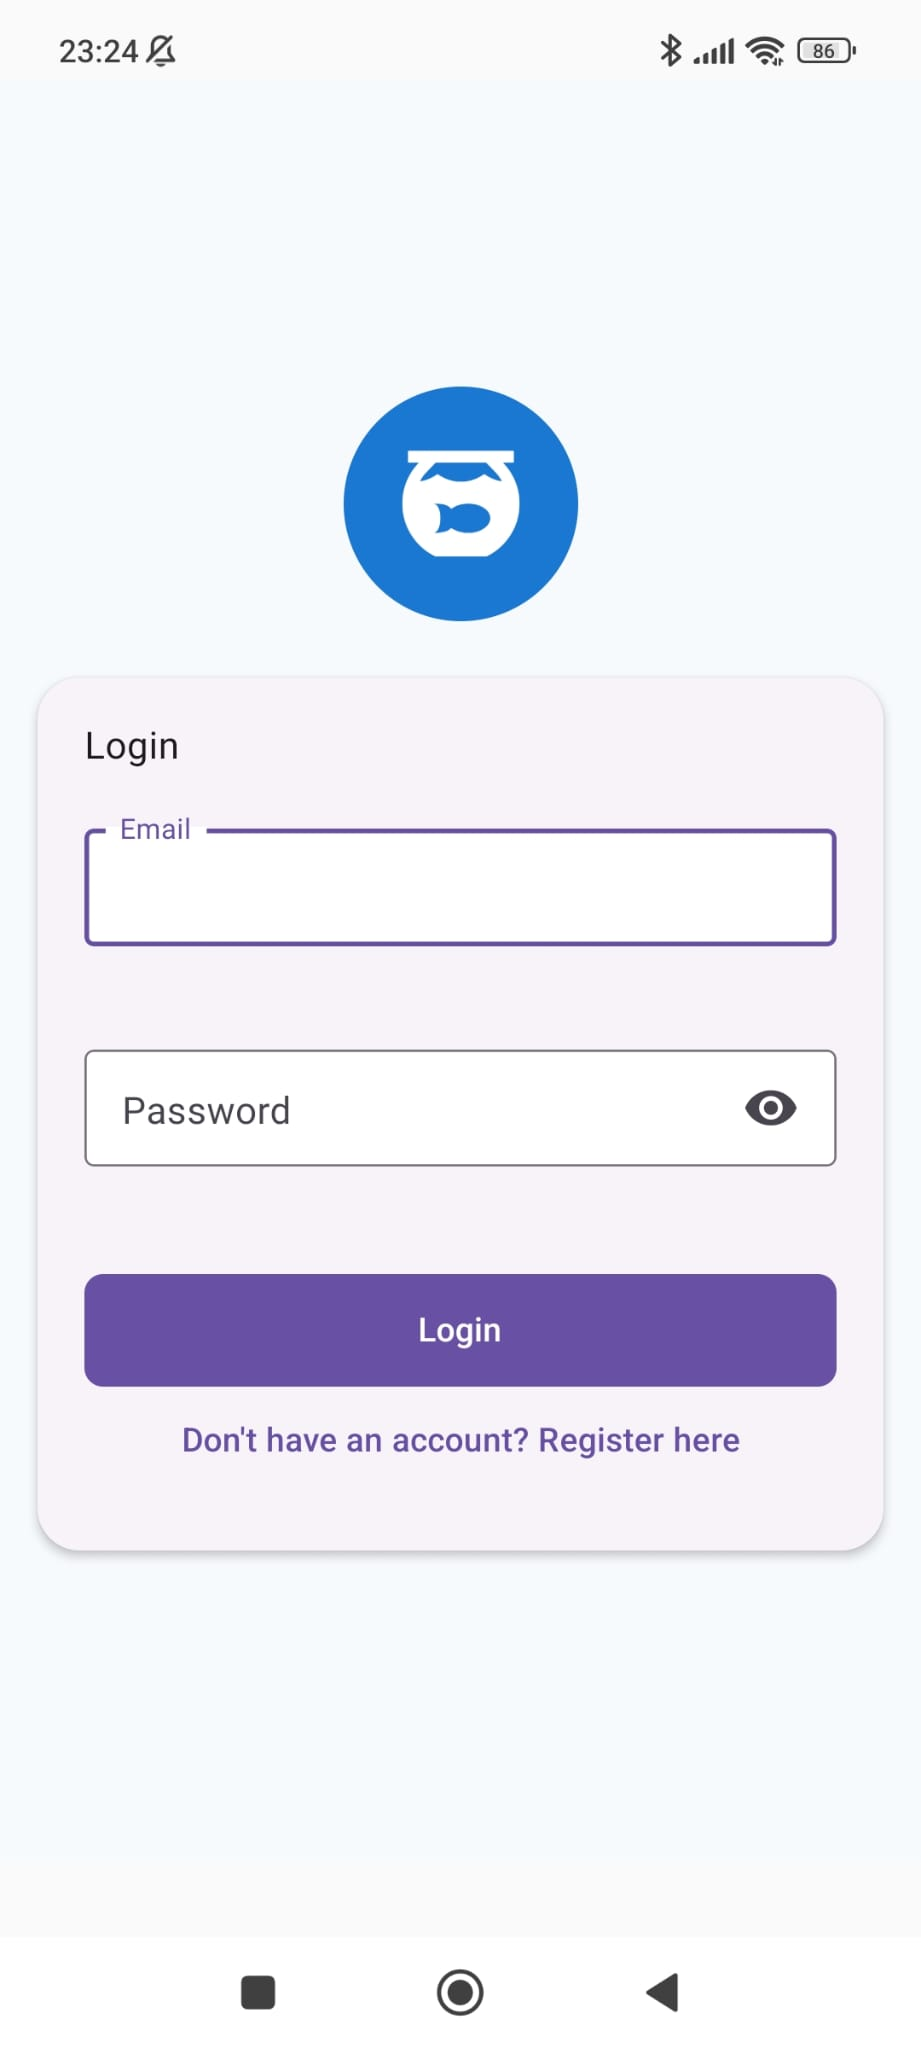
\includegraphics[width=\linewidth]{Images/Login form.jpeg}
        \caption*{Login form}
    \end{minipage}
    \hfill
    \begin{minipage}{0.35\textwidth}
        \centering
        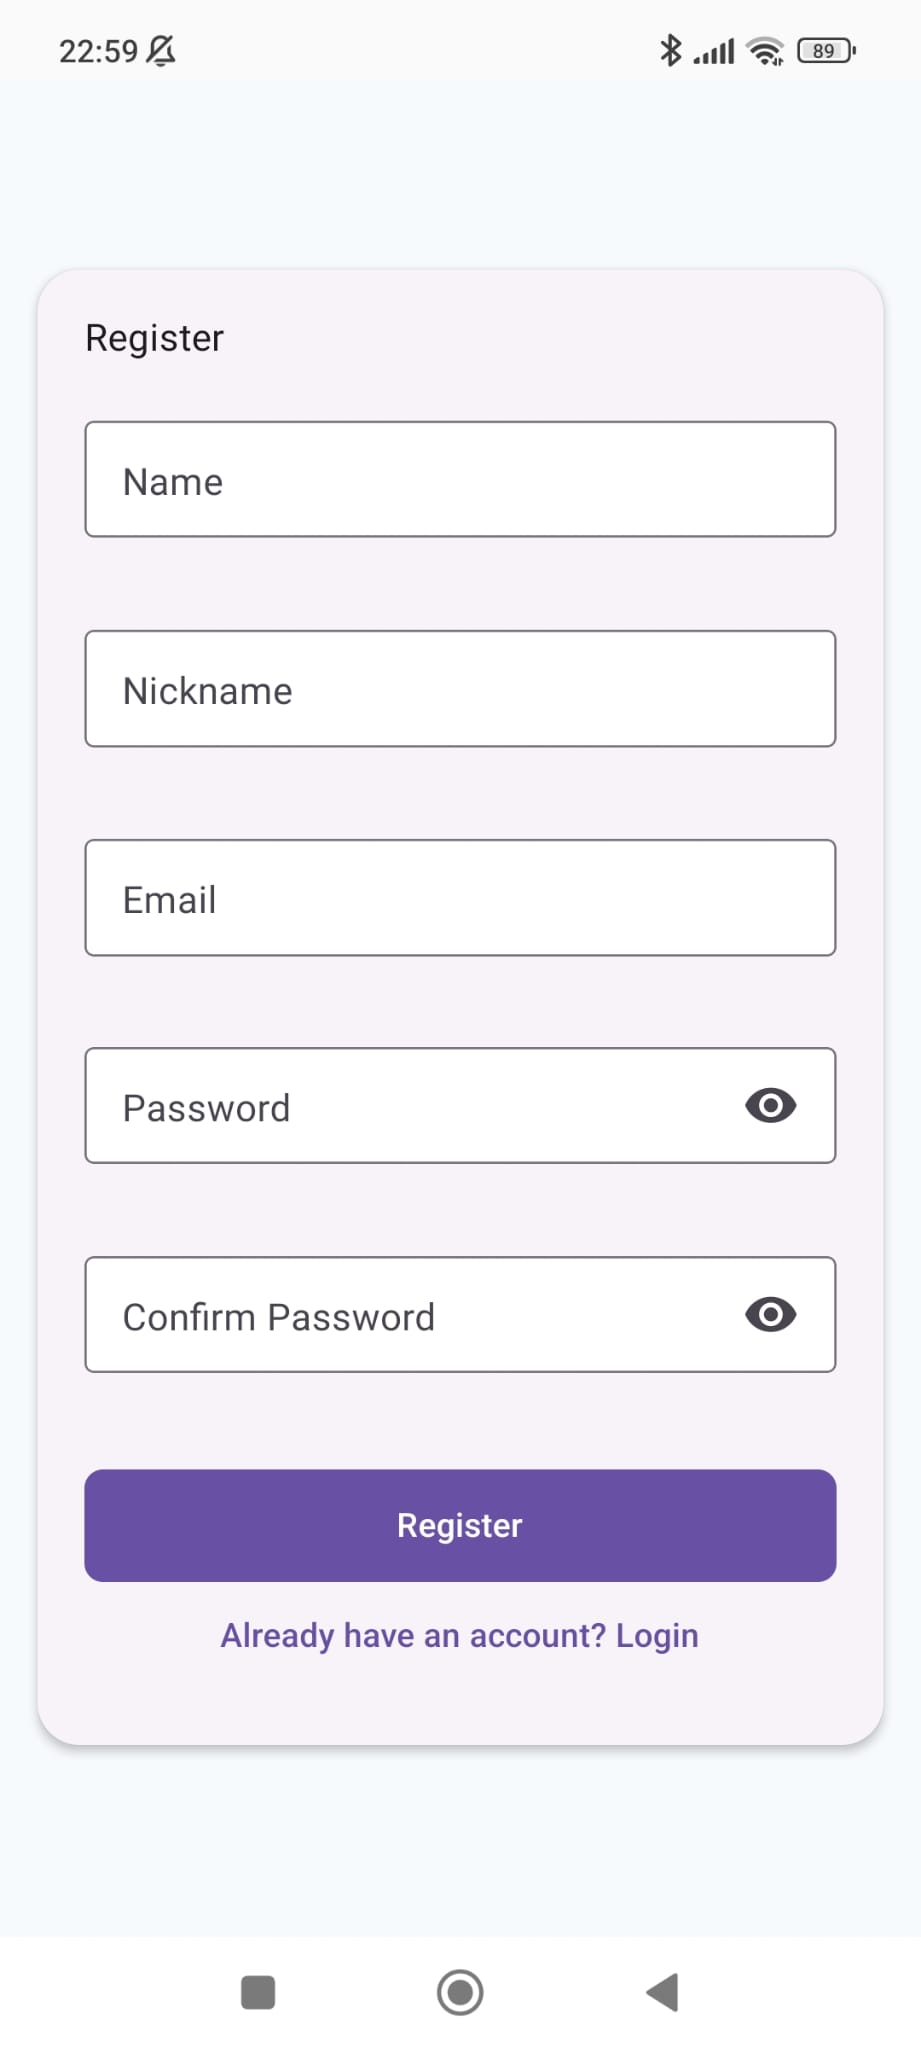
\includegraphics[width=\linewidth]{Images/Register form.jpeg}
        \caption*{Register form}
    \end{minipage}
\end{figure}

\vspace{2em}
When entering the app for the first time, the user is greeted with login and registration pages, allowing them to either sign into an existing account or create a new one to start managing and monitoring their aquariums. Each aquarium is associated with an account, being possible for an aquarium's owner to share it with other users.

\begin{figure}[H]
    \centering
    \begin{minipage}{0.35\textwidth}
        \centering
        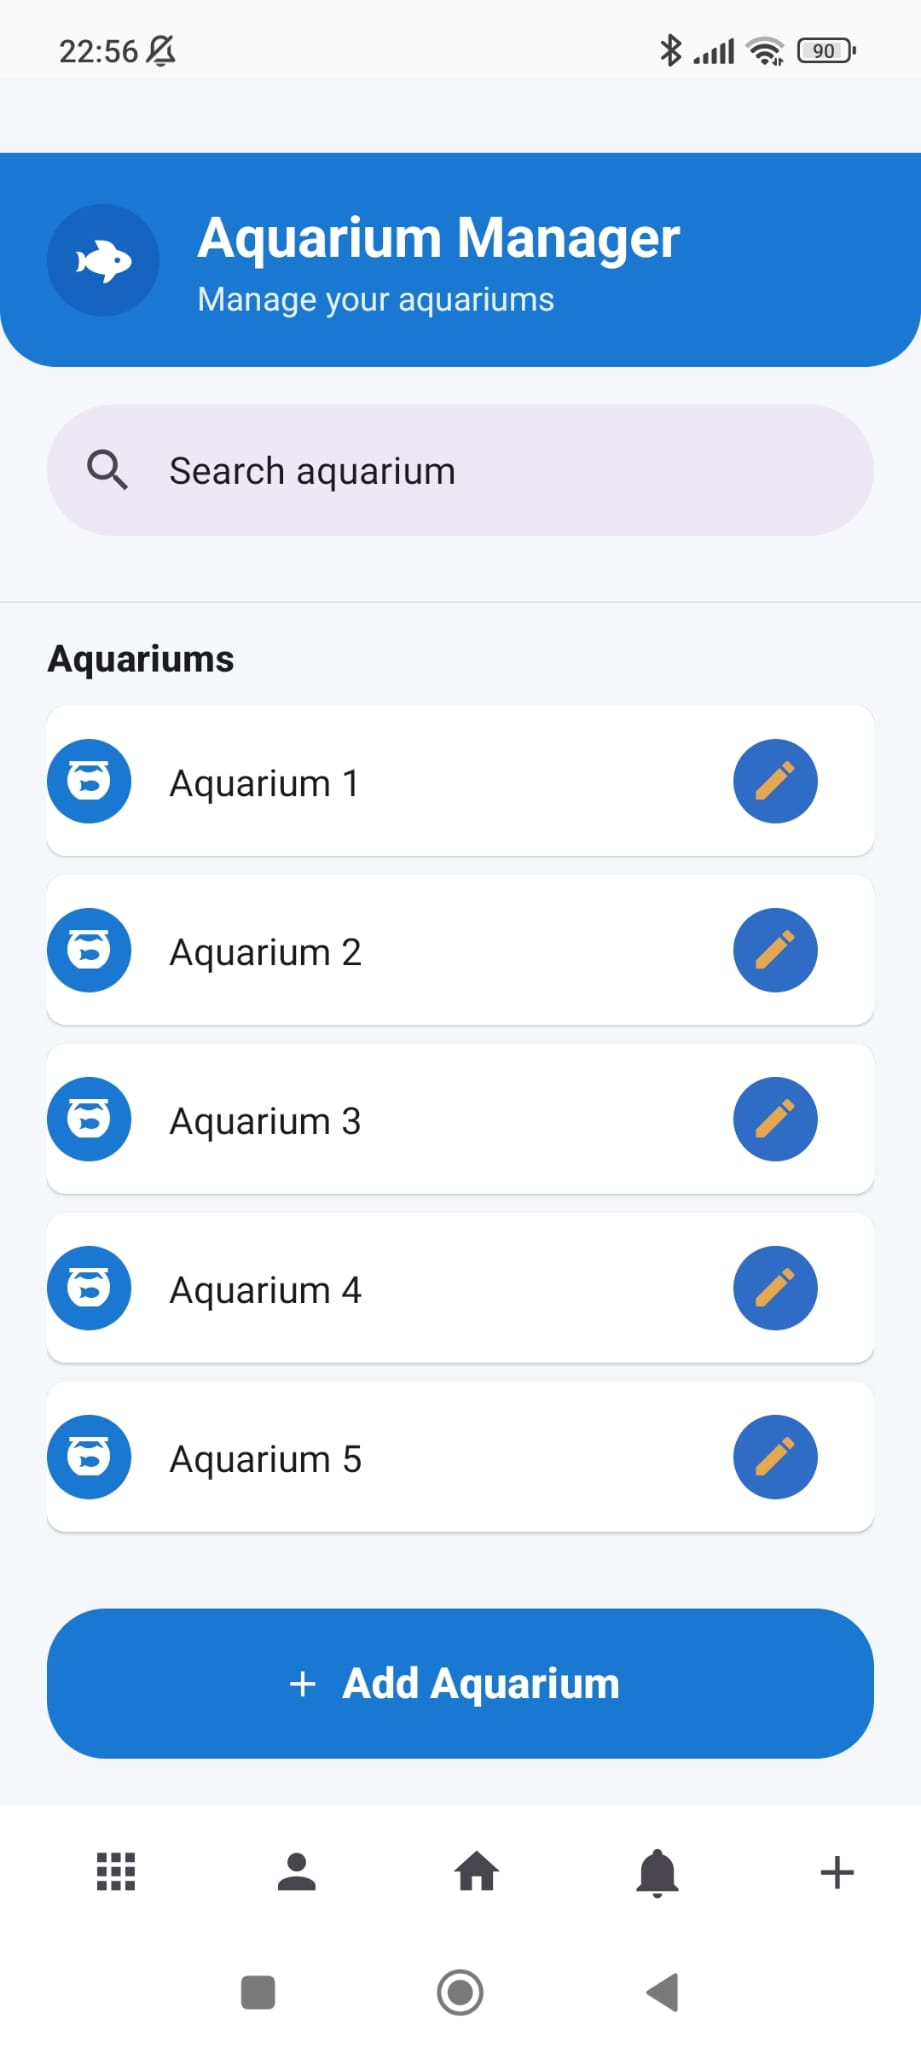
\includegraphics[width=\linewidth]{Images/Homepage.jpeg}
        \caption*{Homepage}
    \end{minipage}
    \hfill
    \begin{minipage}{0.35\textwidth}
        \centering
        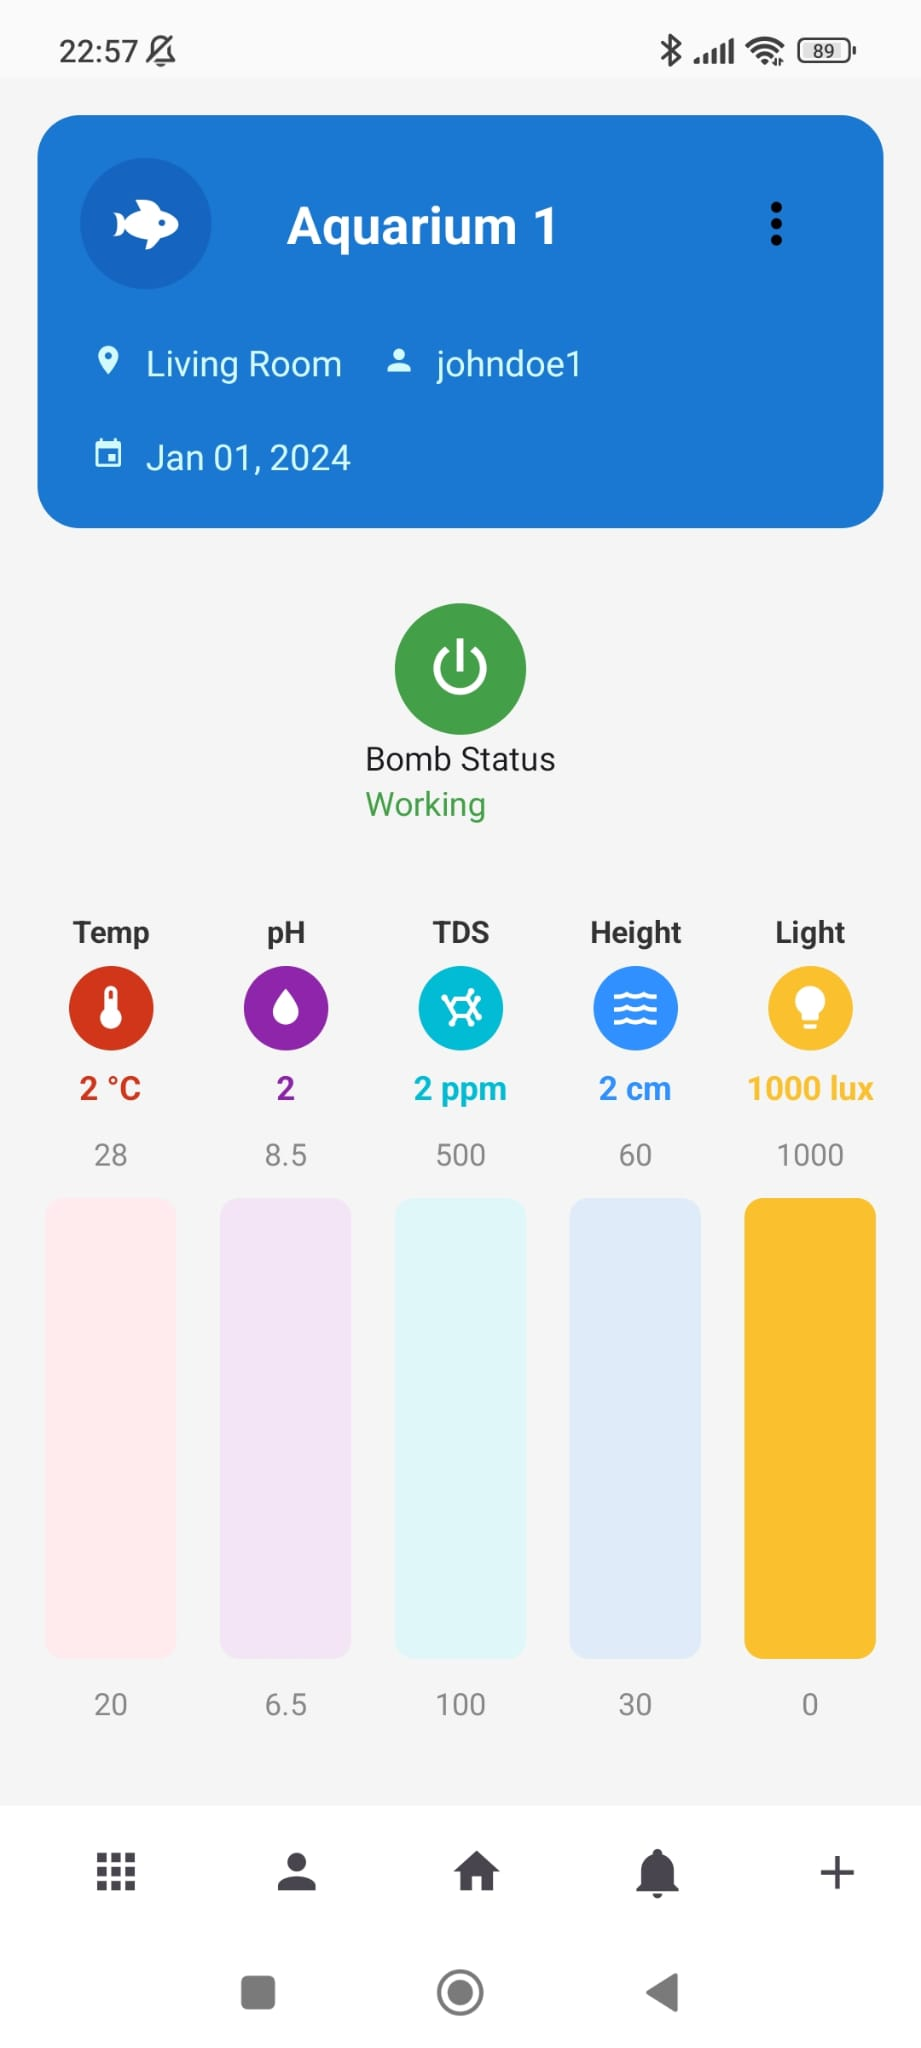
\includegraphics[width=\linewidth]{Images/Aquarium State.jpeg}
        \caption*{Aquarium details and controls}
    \end{minipage}
\end{figure}

\vspace{2em}

Once we log in, we go into the home page that contains the list of our own aquariums and those who we also have view access. We have a search bar that allow us to search for aquariums and we have a "Add Aquarium" button that triggers the flow to register with the esp32.


\begin{figure}[H]
    \centering
    \begin{minipage}{0.35\textwidth}
        \centering
        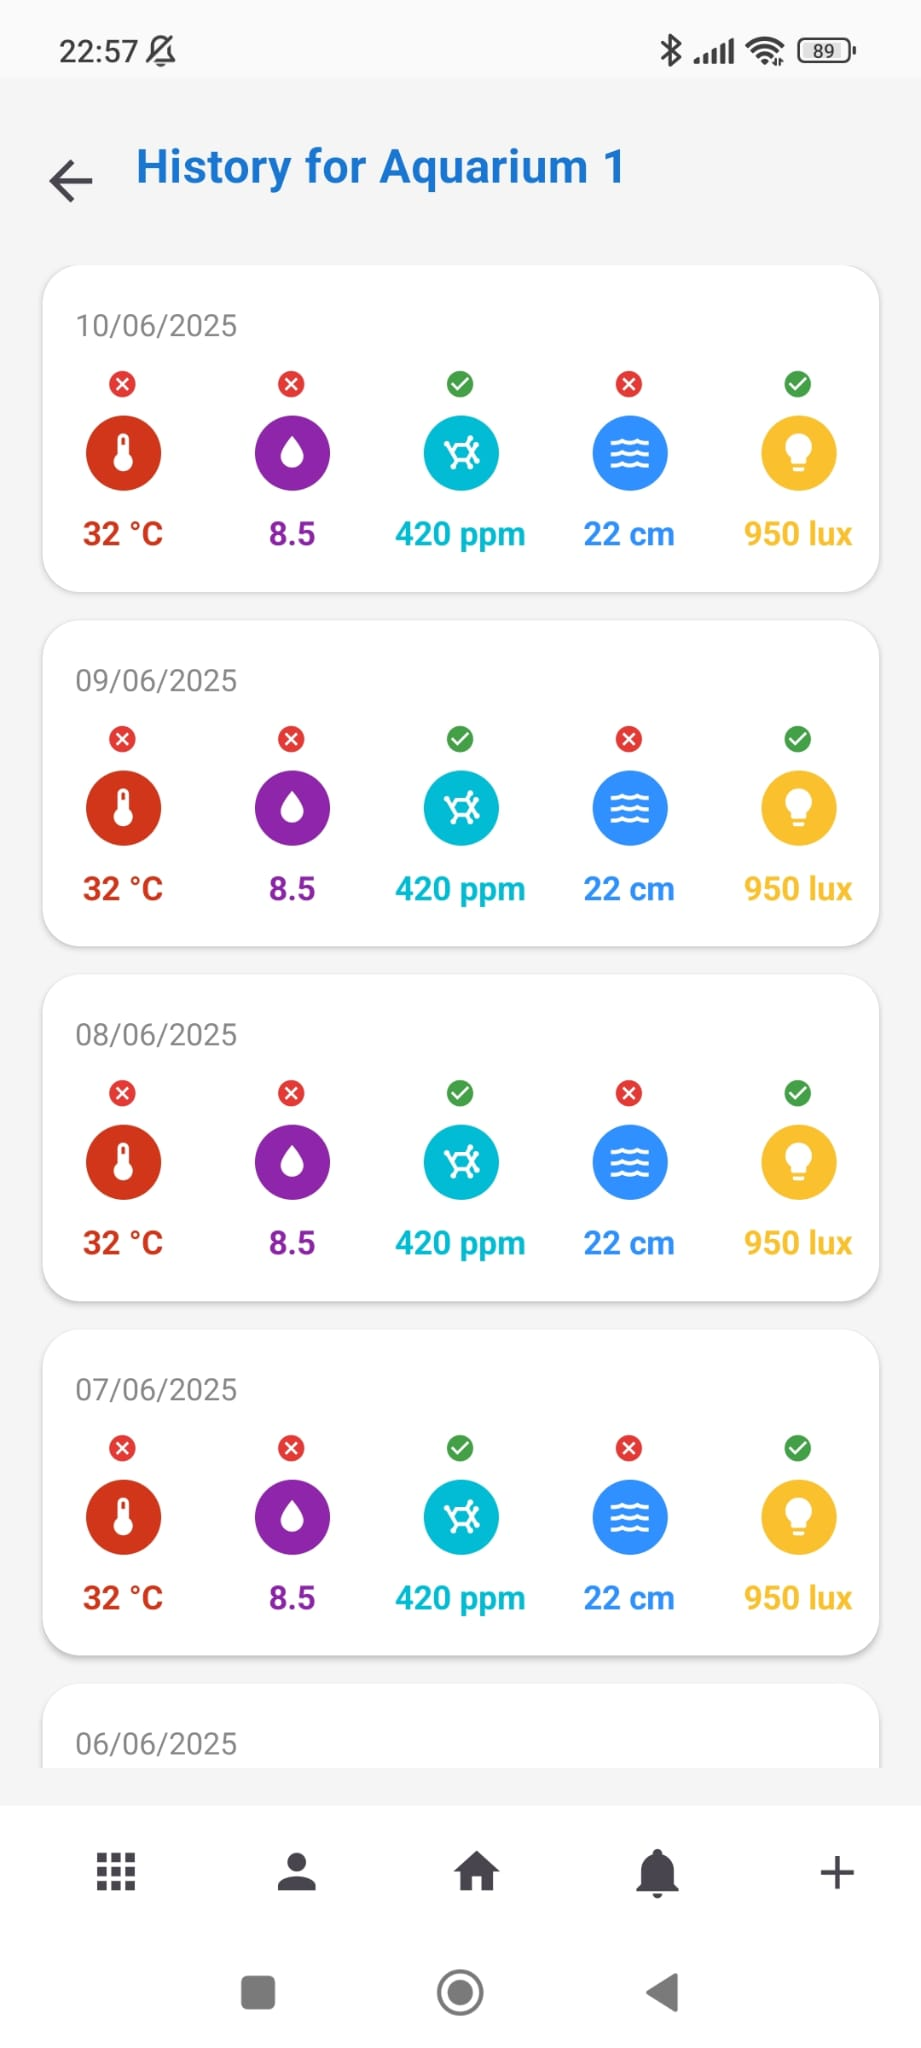
\includegraphics[width=\linewidth]{Images/Aquarium history.jpeg}
        \caption*{Sensor's snapshots history}
    \end{minipage}
    \hfill
    \begin{minipage}{0.35\textwidth}
        \centering
        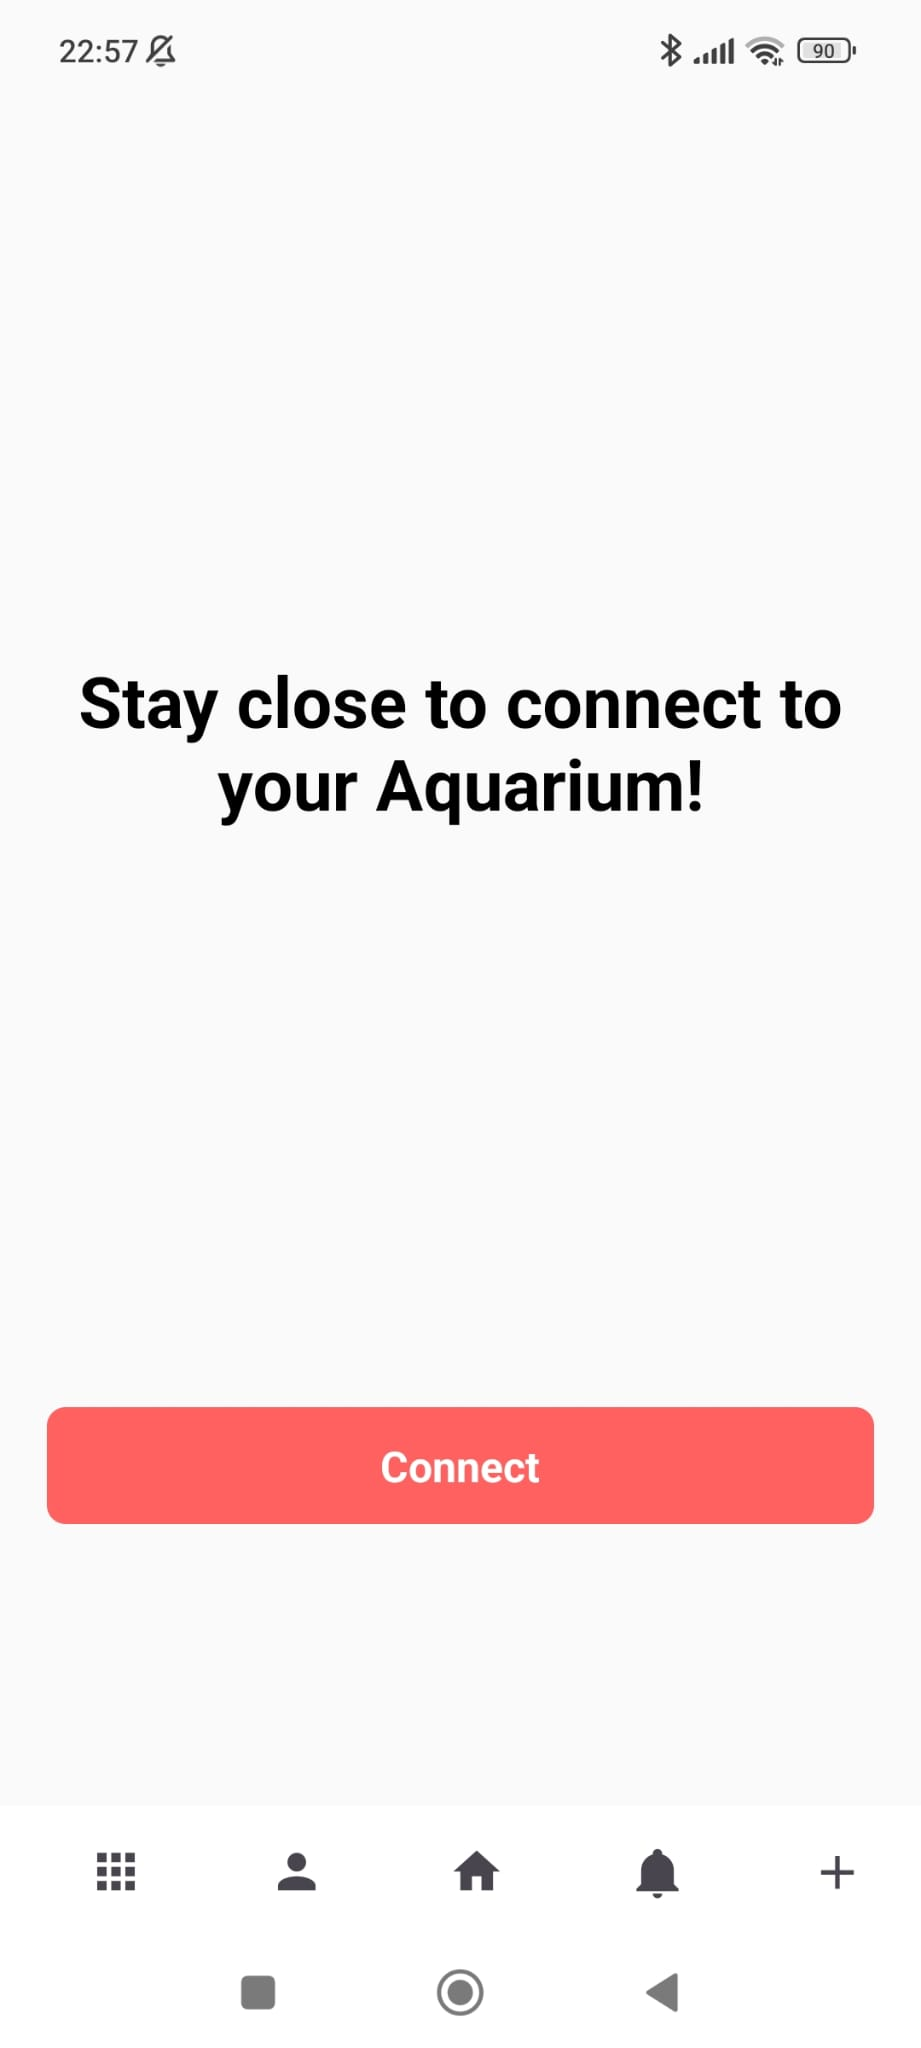
\includegraphics[width=\linewidth]{Images/Connect Aquarium.jpeg}
        \caption*{Pair with Aquarium (ESP32)}
    \end{minipage}
\end{figure}

\vspace{2em}
The system stores sensor snapshots, allowing users to view the historical data for each aquarium and track environmental changes over time. Additionally, the mobile app guides users through the pairing process with a new ESP32 device using Bluetooth, allowing for a simple initial setup.

\begin{figure}[H]
    \centering
    \begin{minipage}{0.35\textwidth}
        \centering
        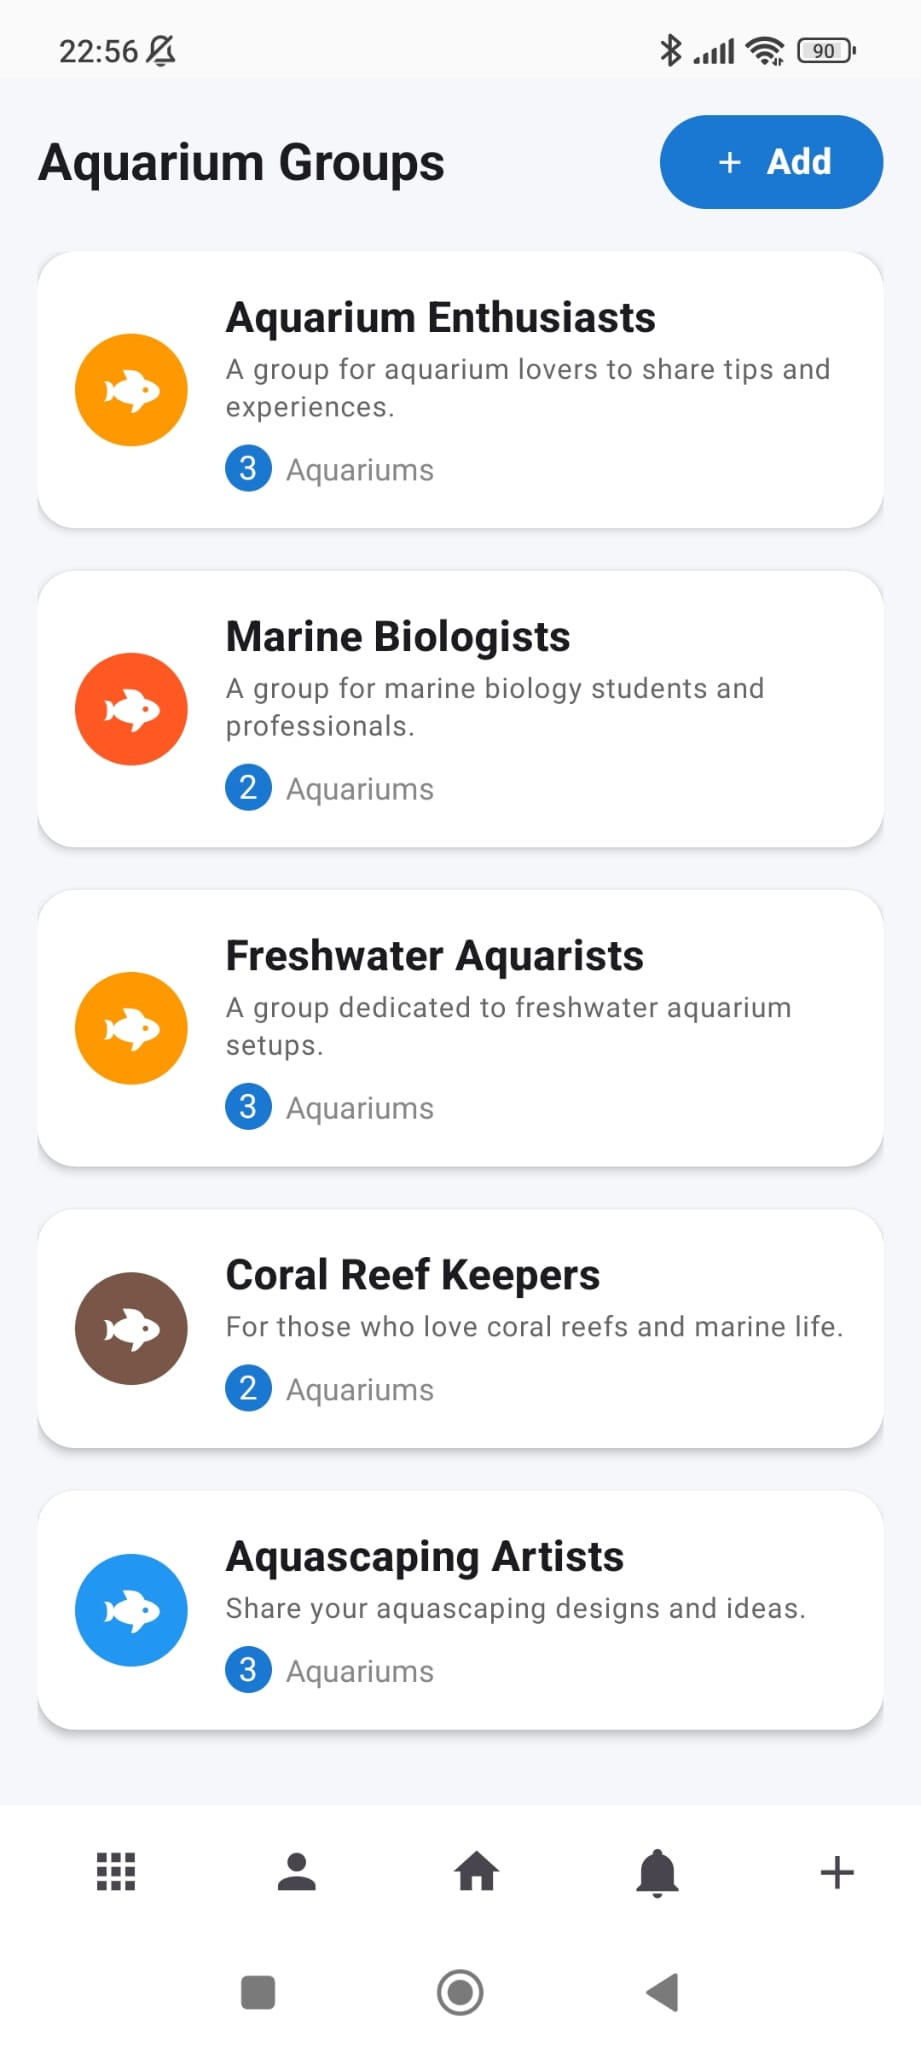
\includegraphics[width=\linewidth]{Images/List groups.jpeg}
        \caption*{Aquarium Groups}
    \end{minipage}
    \hfill
    \begin{minipage}{0.35\textwidth}
        \centering
        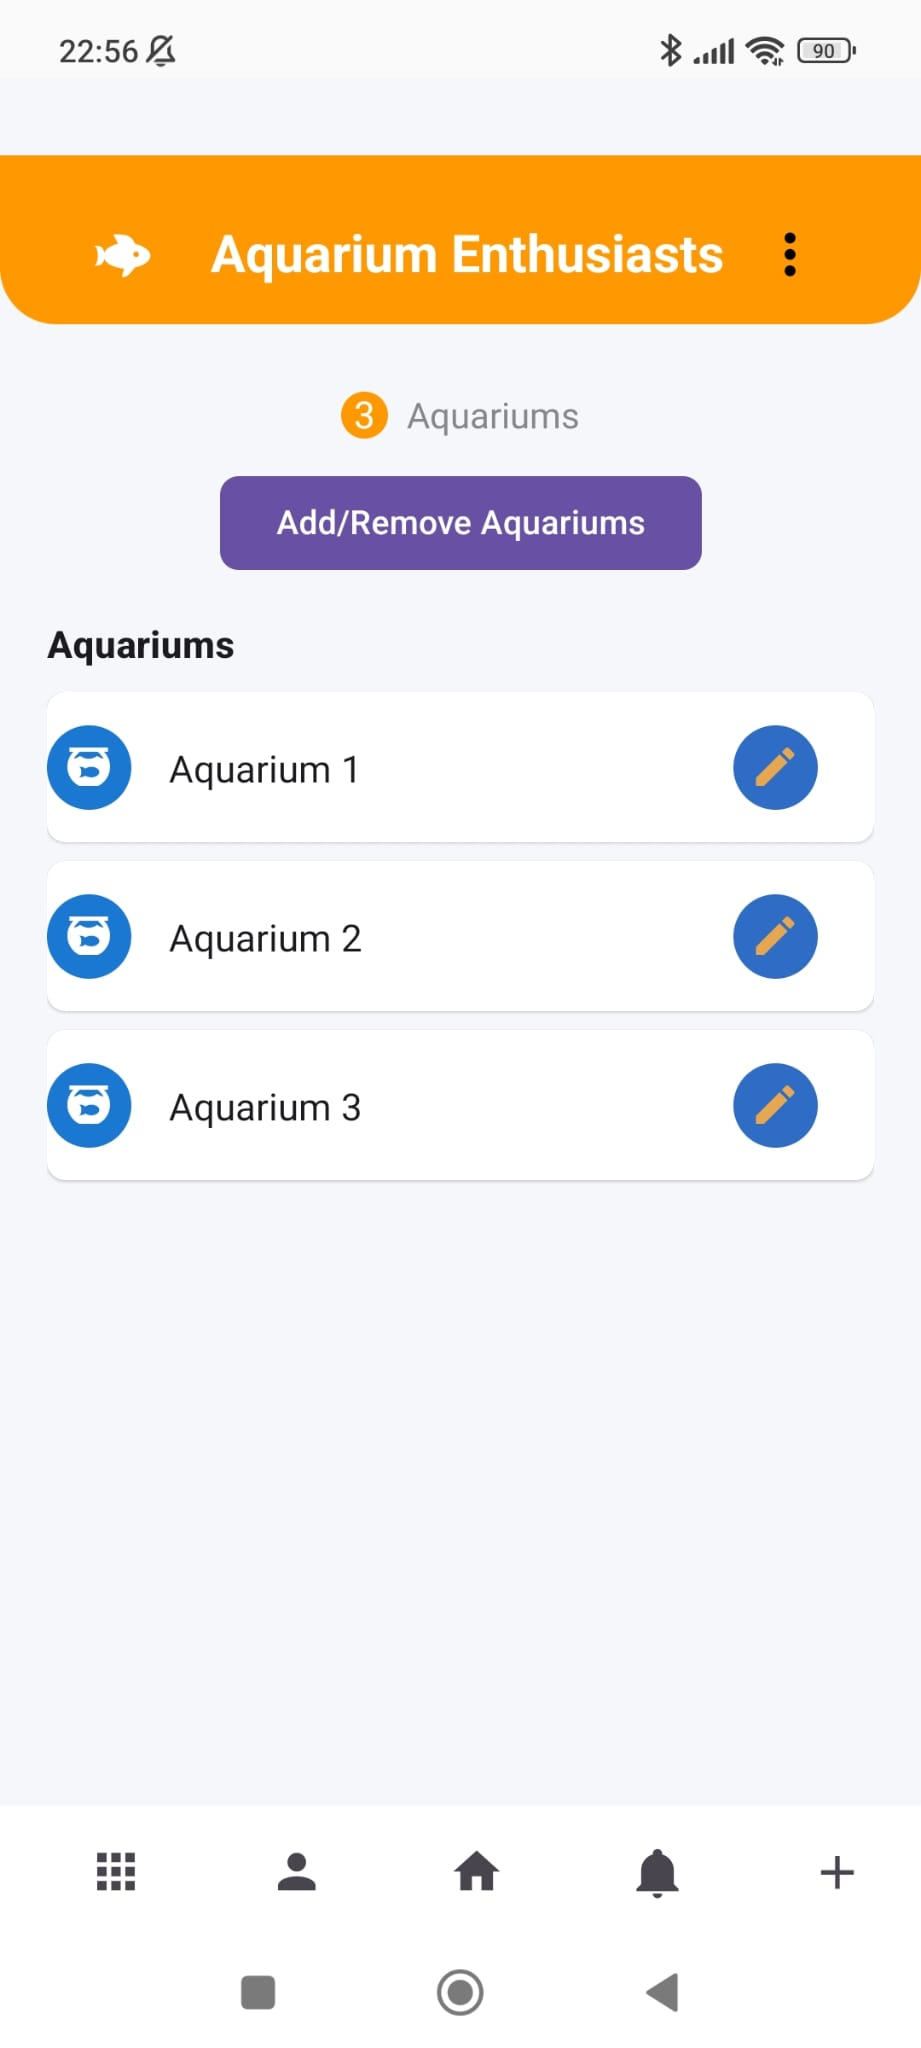
\includegraphics[width=\linewidth]{Images/Aquariums in groups.jpeg}
        \caption*{Add or remove Aquariums in a Group}
    \end{minipage}
\end{figure}

\vspace{2em}
To improve organization and efficiency, the app includes a Groups feature, which allows users to categorize aquariums into shared spaces. This can be useful for grouping aquariums from a specific pet shop or organizing them by fish type or environmental conditions.

\begin{figure}[H]
    \centering
    \begin{minipage}{0.35\textwidth}
        \centering
        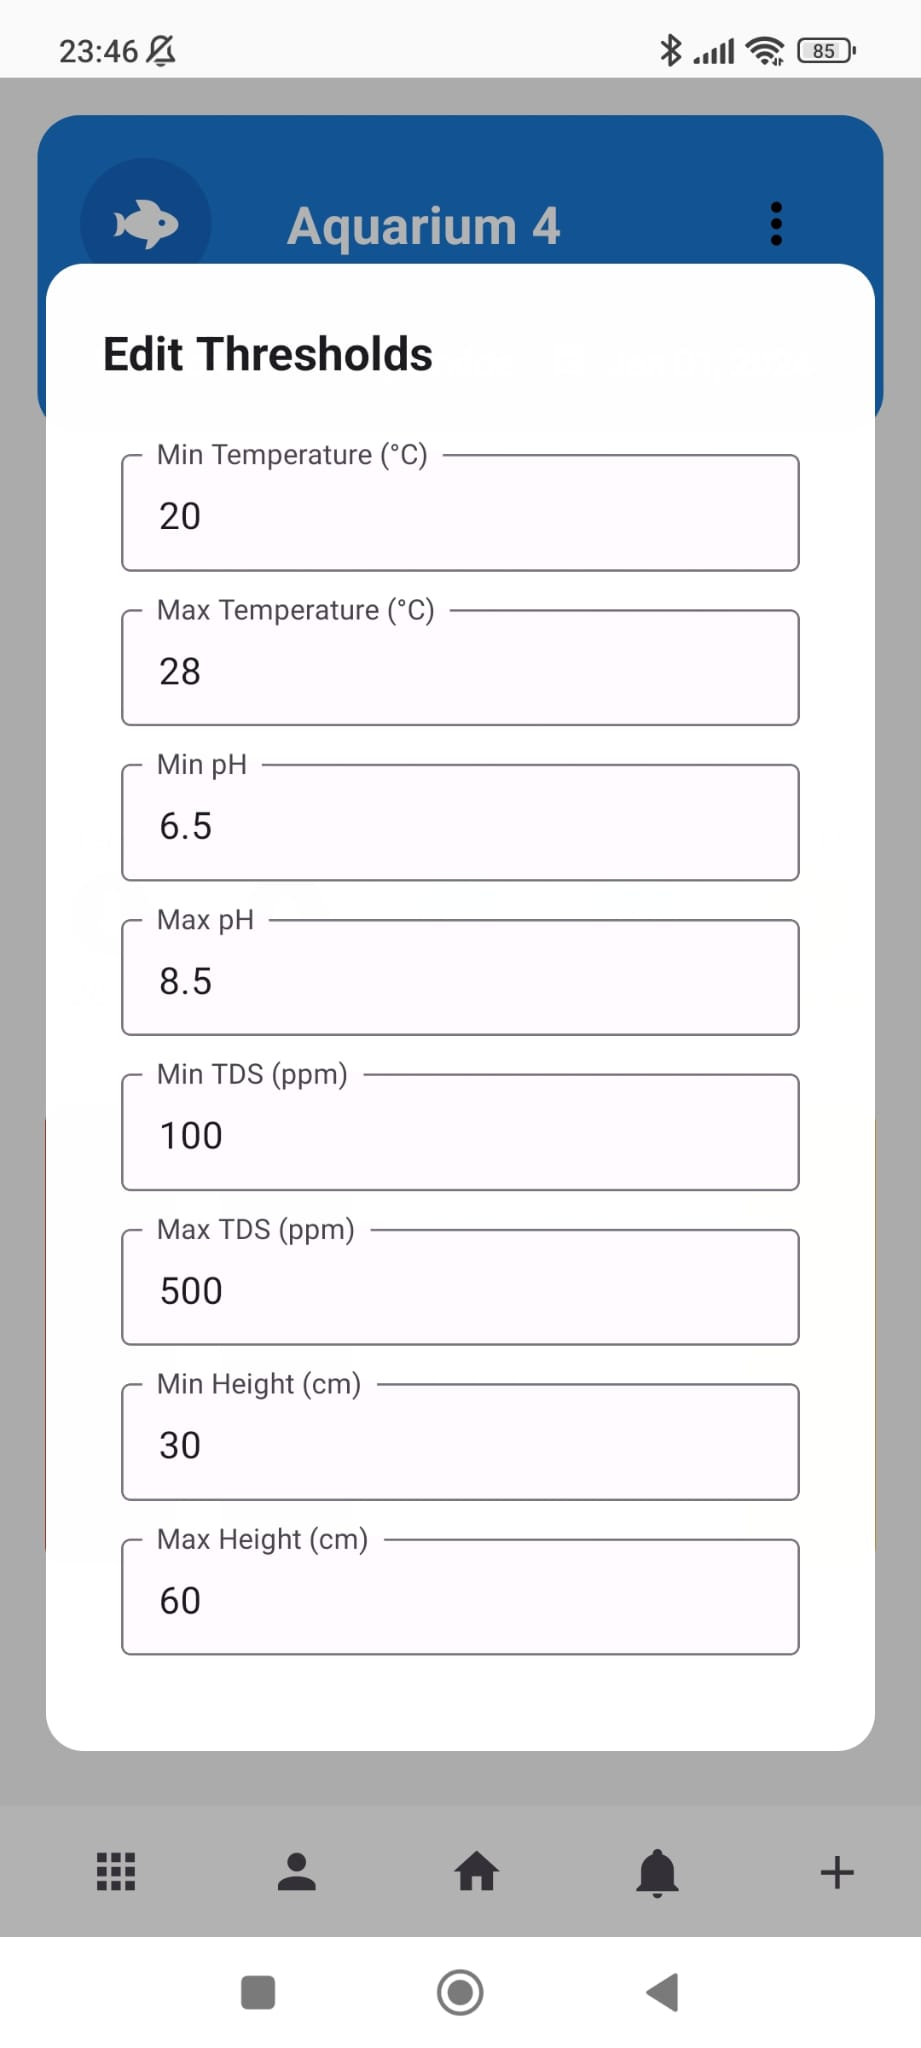
\includegraphics[width=\linewidth]{Images/thresholds.jpeg}
        \caption*{Edit Aquarium Thresholds}
    \end{minipage}
    \hfill
    \begin{minipage}{0.35\textwidth}
        \centering
        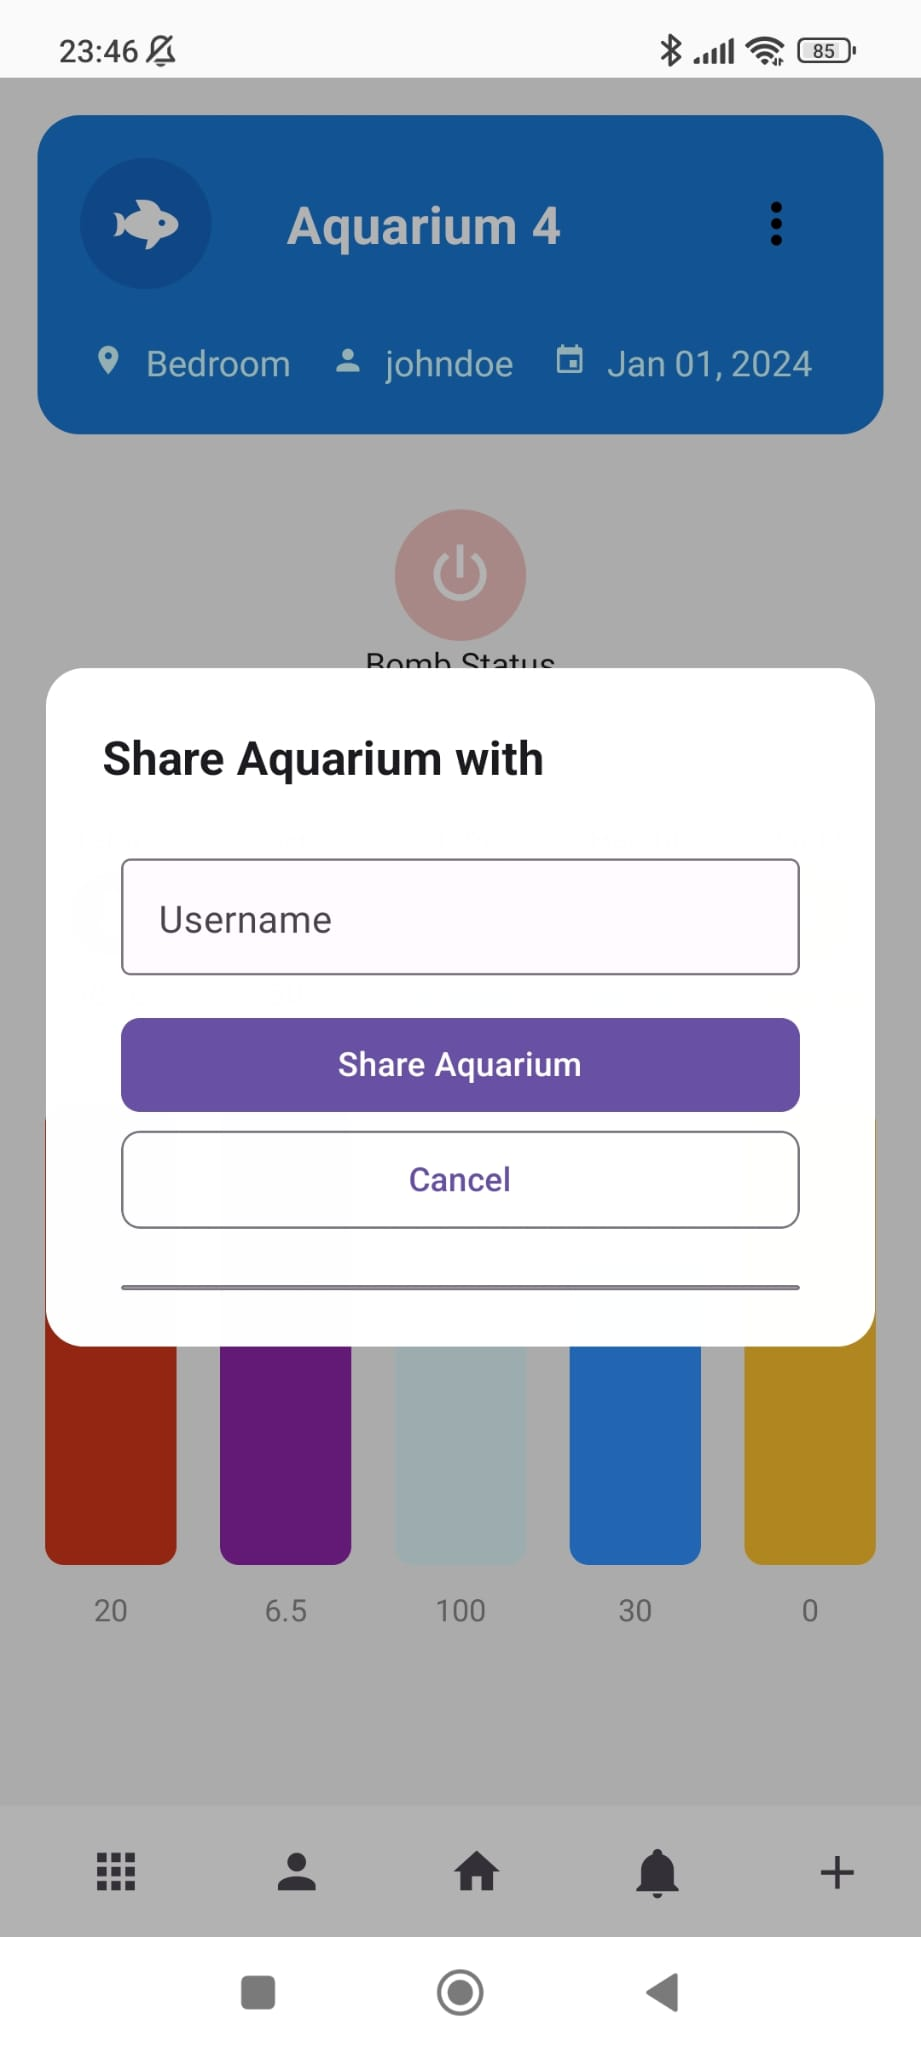
\includegraphics[width=\linewidth]{Images/share.jpeg}
        \caption*{Share Aquarium}
    \end{minipage}
\end{figure}

\vspace{2em}
Each aquarium has configurable threshold values for parameters such as temperature, pH, TDS, light and water level. These thresholds determine when the system triggers warnings or automatic actions. Additionally, users can easily share aquariums with others by entering their username, allowing for collaborative monitoring and management.

\pagebreak

\section{Sensing and Reacting}

The system continuously monitors the aquarium environment using various sensors. The TDS (Total Dissolved Solids) sensor measures the concentration of dissolved substances in the water, while the temperature sensor tracks the water temperature. The pH sensor monitors the acidity or alkalinity of the water, and the ultrasonic sensor measures the water level. The LDR (Light Dependent Resistor) sensor detects ambient light levels.

When any sensor reading exceeds predefined thresholds, the system reacts by activating the buzzer to alert the user. Additionally, if the TDS level is too high, the water pump will automatically turn on, to refill the aquarium and clear the water. Alternatively, the user can turn on or off the water pump, through a button in the mobile application.

\subsection{Waiting screen}

\begin{figure}[h!]
    \centering
    \begin{minipage}{0.25\textwidth}
        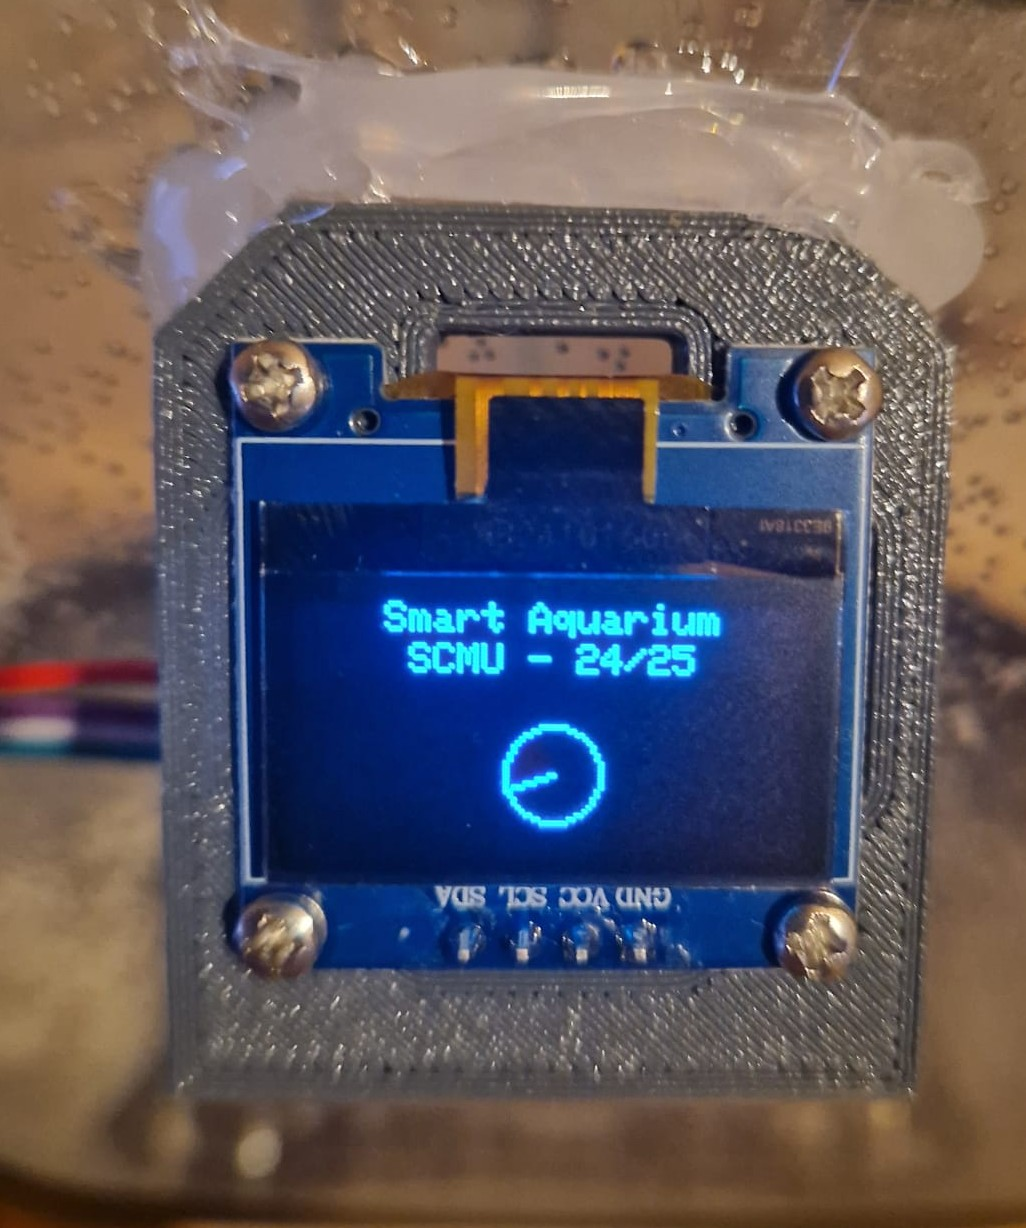
\includegraphics[width=\linewidth]{Images/clock.jpeg}
    \end{minipage}%
    \hfill
    \begin{minipage}{0.55\textwidth}
        \small
        For better user experience using the aquarium, the OLED display shows a little clock while the user is completing the initial setup. This is done to avoid having a blank screen while the user is waiting for the BLE and Wi-Fi connection to be established.

        This is done using two threads: one for the setup and another for the clock. The clock thread updates the OLED display every second.
    \end{minipage}
\end{figure}

\subsection{Saving Wi-Fi credentials}

The initial setup of the system requires the user to provide Wi-Fi credentials to connect the microcontroller to the internet. This is done using Bluetooth Low Energy (BLE) for secure and efficient communication with the mobile application.

When the ESP32 receives the Wi-Fi credentials from the mobile app, it saves them in non-volatile memory (NVM) using the \href{https://github.com/vshymanskyy/Preferences}{Preferences library} to ensure they persist across reboots. This allows the microcontroller to automatically reconnect to the Wi-Fi network without requiring user intervention each time it starts up.

\pagebreak

\section{Experiments}

During the development of the Smart Aquarium system, we conducted several experiments to validate the functionality and performance of the hardware and software components. These experiments focused on sensor accuracy, actuator responsiveness, and overall system reliability.

Each sensor was tested individually to ensure it provided accurate readings.

\subsection{Final prototype}

\begin{figure}[h!]
    \centering
    \begin{minipage}{0.35\textwidth}
        \centering
        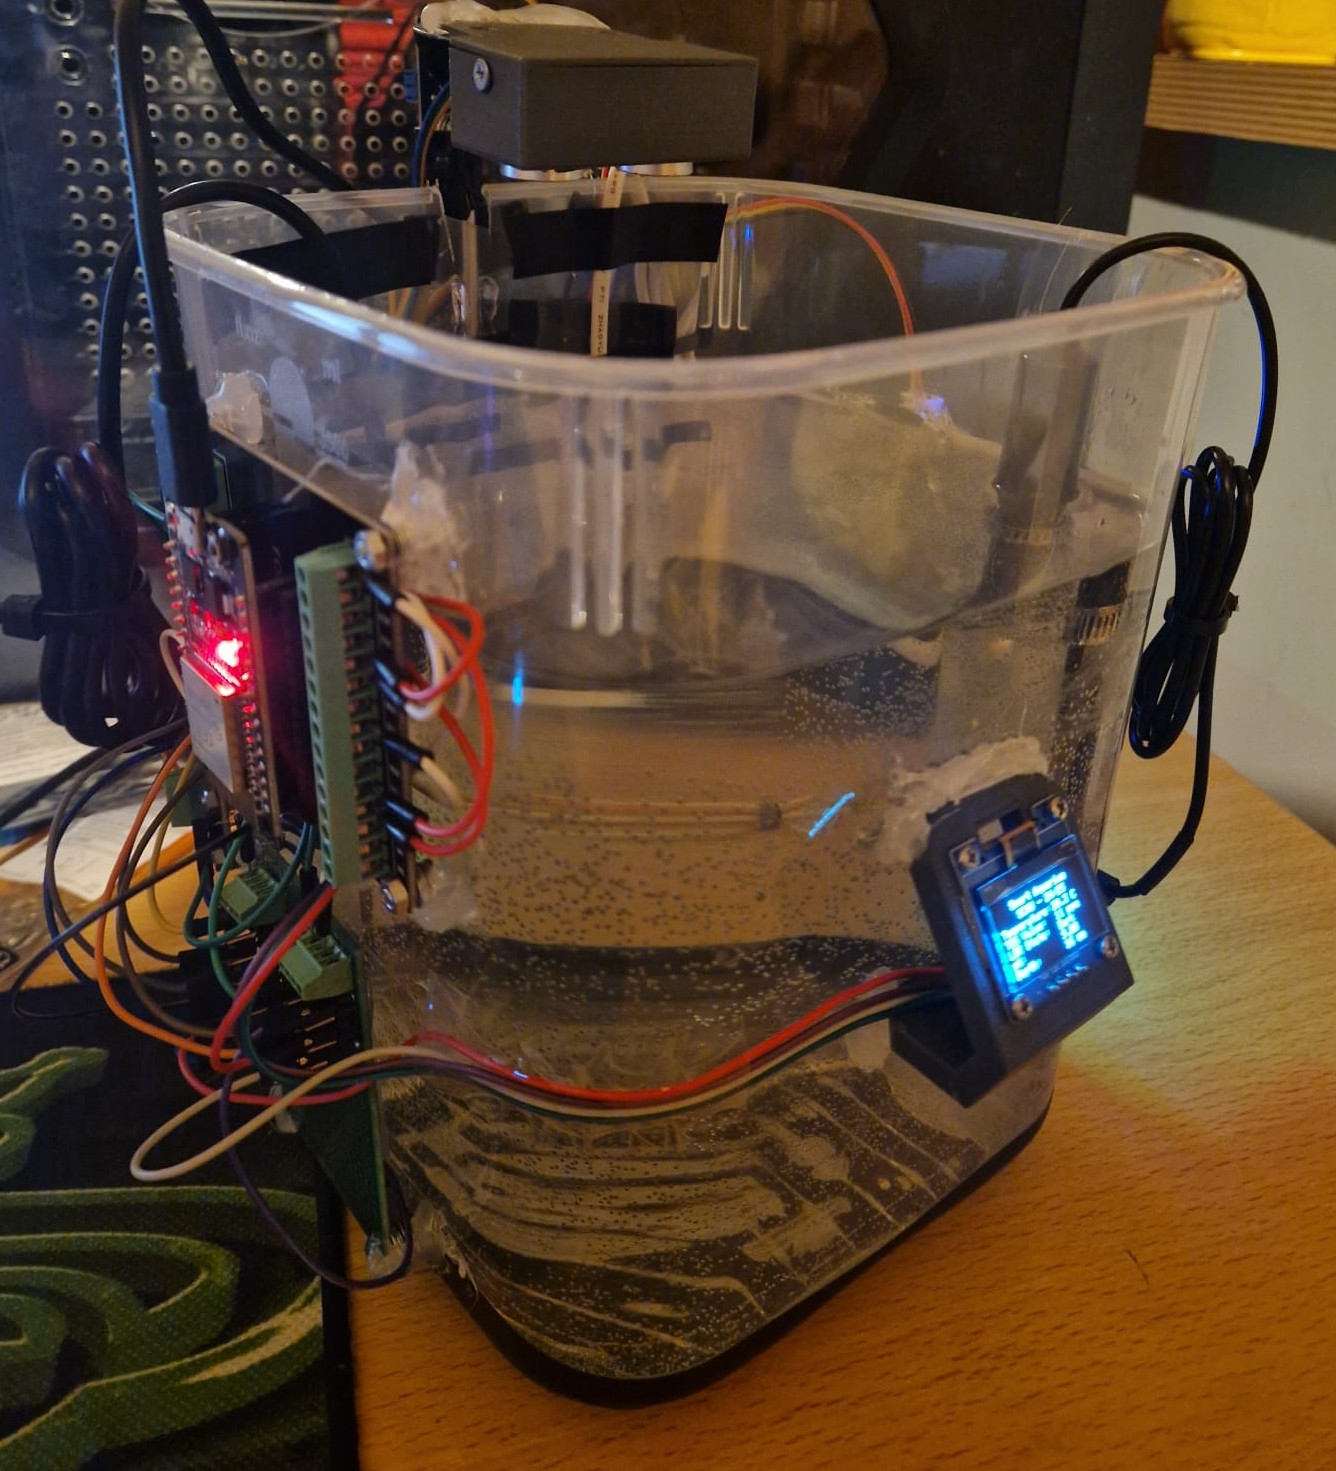
\includegraphics[width=\linewidth]{Images/frenteProt.jpeg}
    \end{minipage}
    \hfill
    \begin{minipage}{0.33\textwidth}
        \centering
        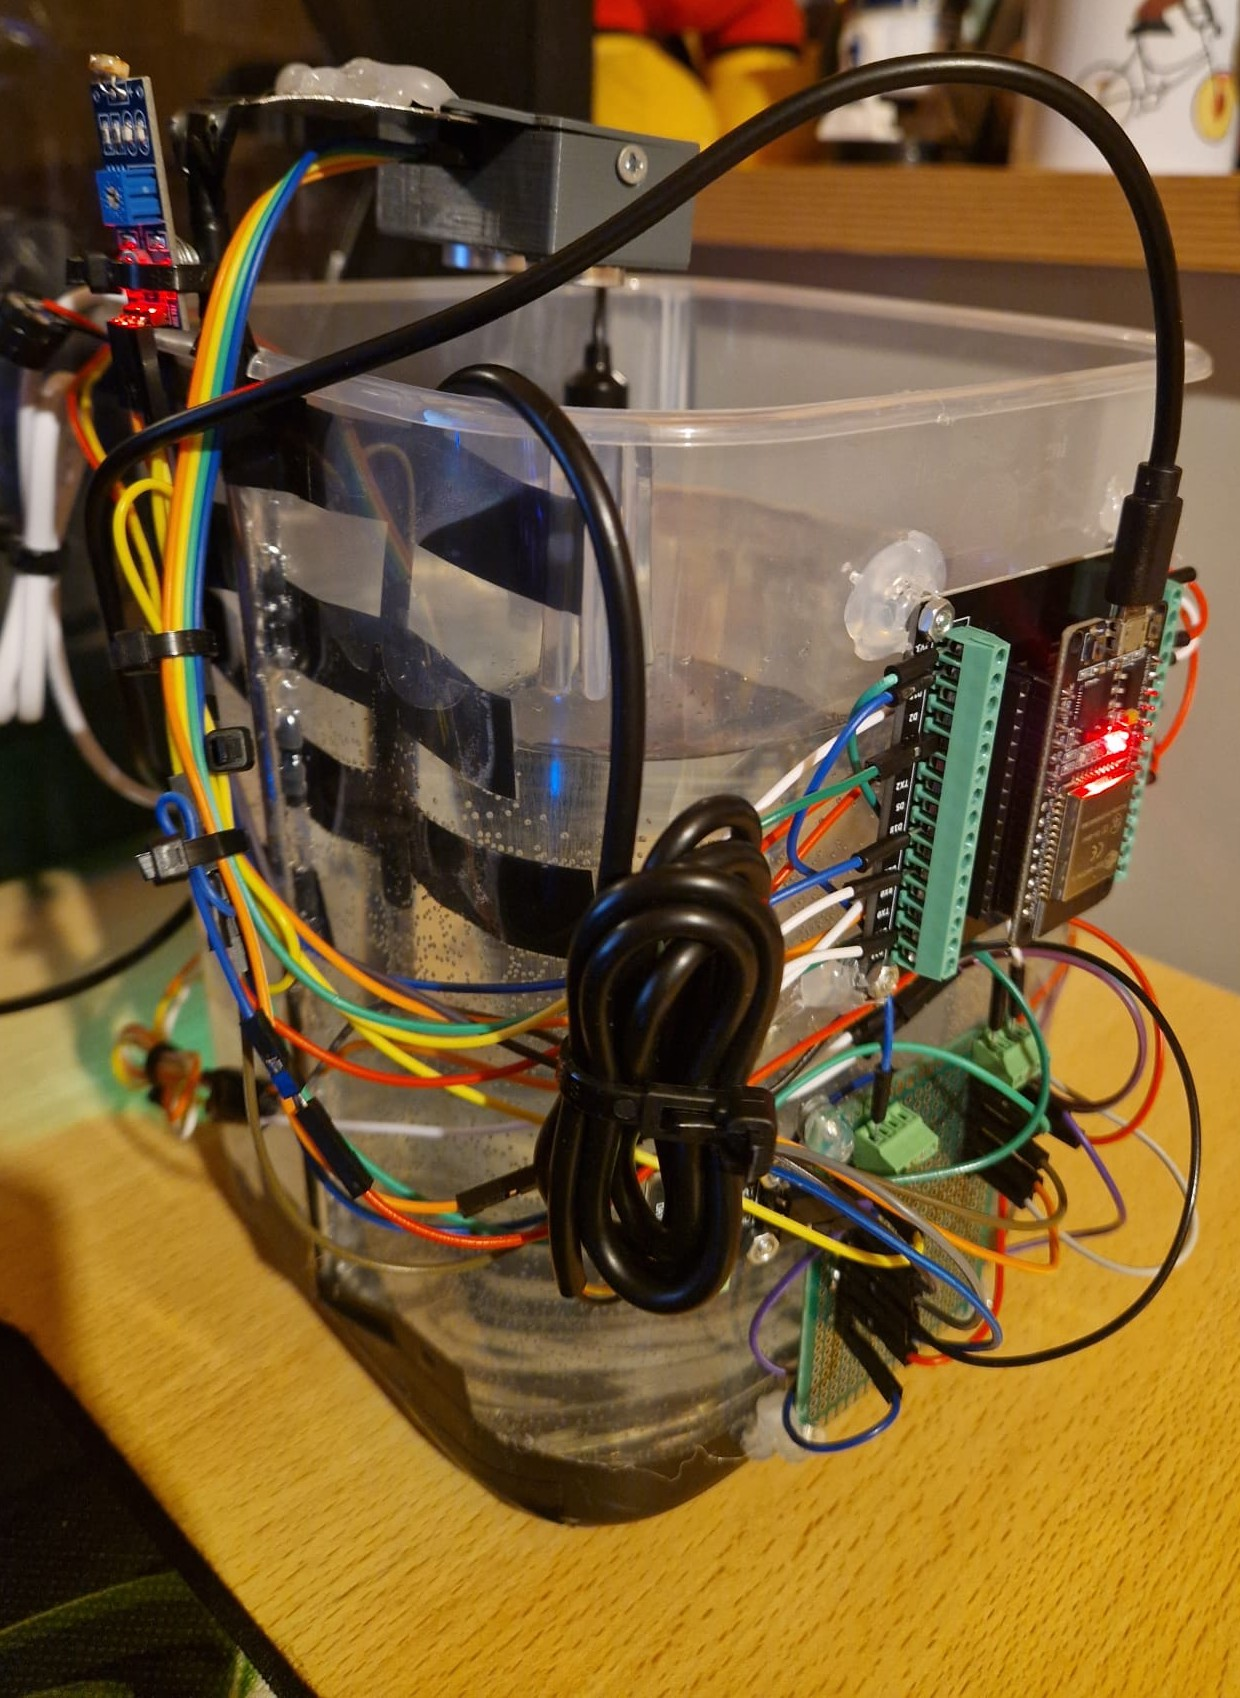
\includegraphics[width=\linewidth]{Images/trasProt.jpeg}
    \end{minipage}
\end{figure}

\begin{figure}[h!]
    \centering
    \begin{minipage}{0.35\textwidth}
        \centering
        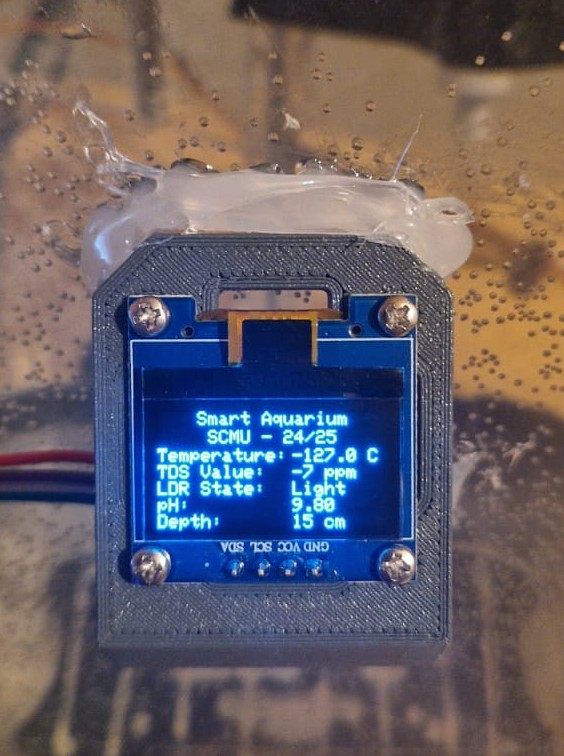
\includegraphics[width=\linewidth]{Images/disp.jpeg}
    \end{minipage}
    \hfill
    \begin{minipage}{0.35\textwidth}
        \centering
        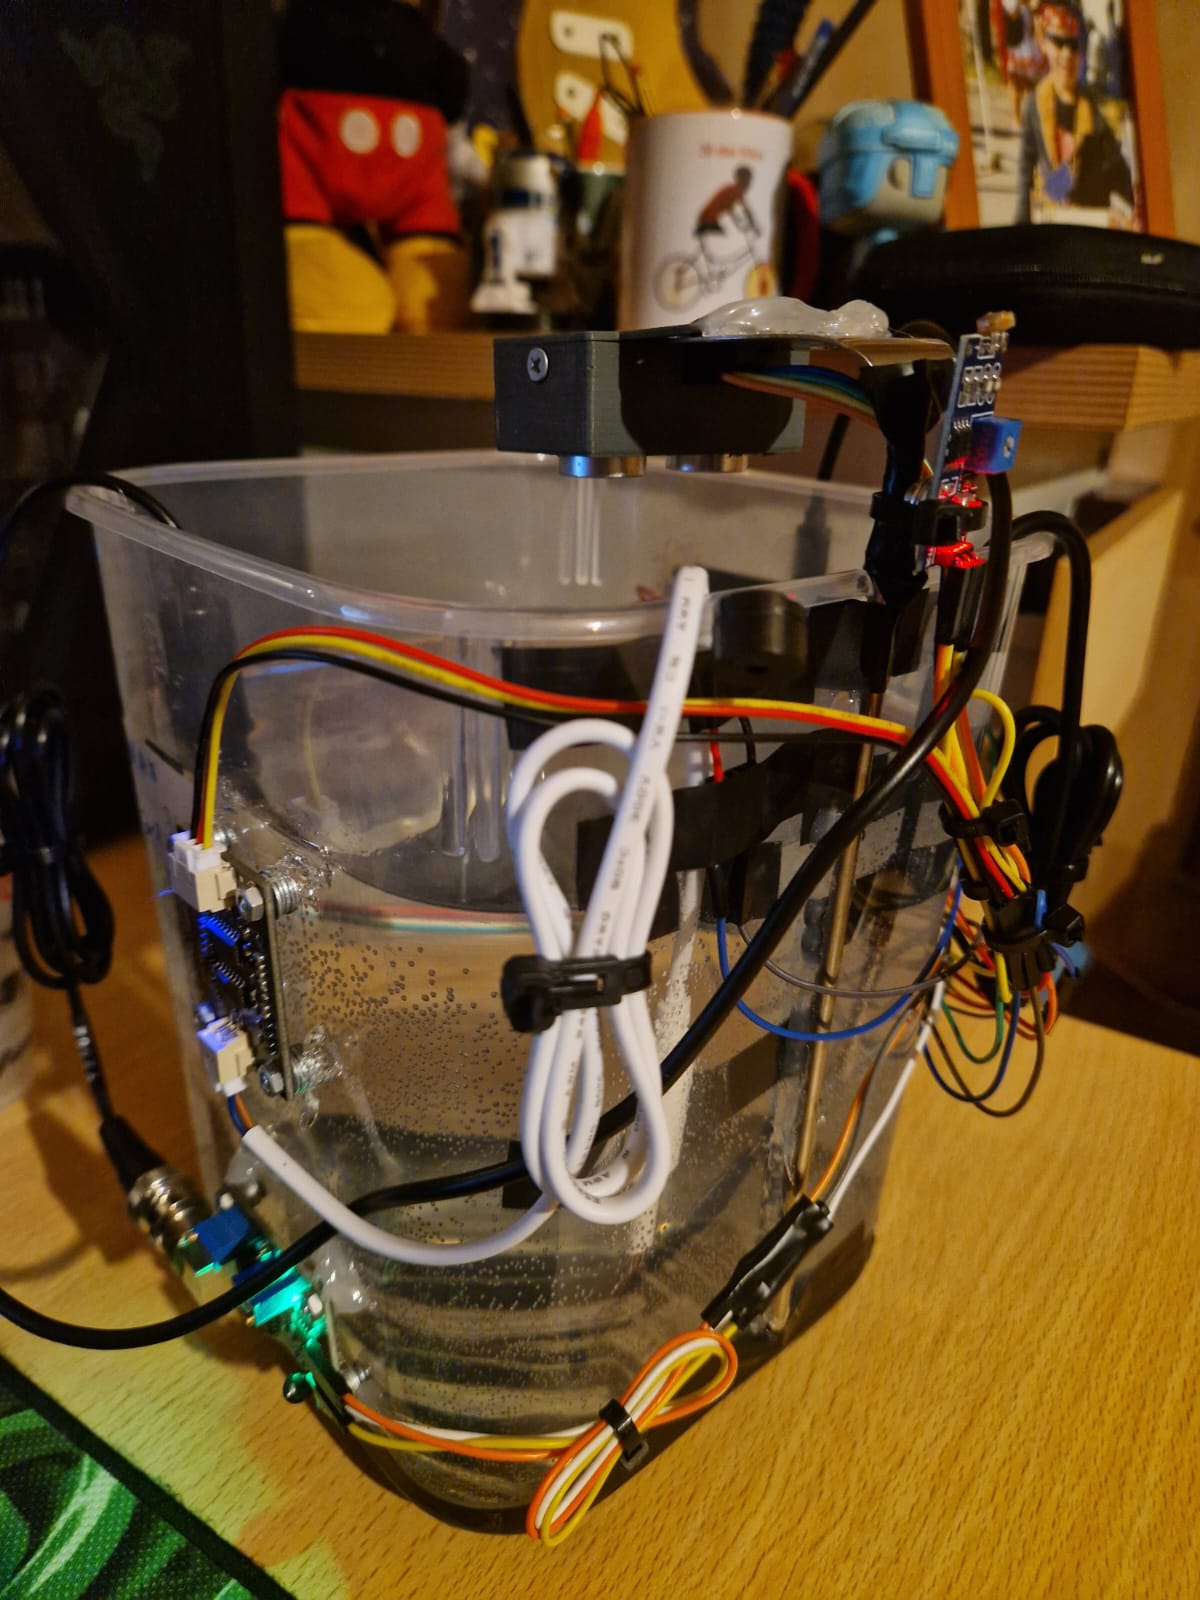
\includegraphics[width=\linewidth]{Images/tras2Prot.jpeg}
    \end{minipage}
\end{figure}

\pagebreak

\section{Conclusions and Lessons Learned}

This project demonstrated the potential of using ESP32 microcontrollers to create a smart, compact and automated system. In a real-world deployment, key areas to improve would include better security, support for firmware updates over the air and explore GPS capabilities that could be used in the hardware.

One of the main lessons learned was the effectiveness of using BLE for initial configuration and the importance of reliable communication within services. We also gained practical experience in sensor integration, actuator control, and real-time data handling on resource-constrained devices. Overall, the ESP32 proved to be a powerful and flexible platform for IoT development.

\end{document}